\documentclass[10pt]{article}
\textwidth 16.5cm
\textheight 25.5cm
\oddsidemargin 0pt
\topmargin -3cm
% \usepackage{epsf}

% Draft watermark
\usepackage[
stamp = false,
firstpageonly = true
]{draftwatermark}

% Font and formatting
\usepackage[default]{lato}
\usepackage[skip=3pt]{parskip}
% \usepackage{titlesec}
% \titlespacing{\paragraph}{0pt}{*1}{*2}

 \usepackage[compact]{titlesec} 

% Writing maths
\usepackage{
    amsmath, % aligns, equations, etc.
    amsfonts, % blackboard bold, etc.
    bbm, % blackboard bold for numbers.
}

% Figures
\usepackage{graphicx}
\usepackage{floatrow}
\floatsetup[table]{capposition=top}
\newcommand*{\figuretitle}[1]{%
    {\centering%   <--------  will only affect the title because of the grouping (by the
    \textbf{#1}%              braces before \centering and behind \medskip). If you remove
    \par\medskip}%            these braces the whole body of a {figure} env will be centered.
}

% Boxes
\usepackage{enumitem}
\usepackage{tcolorbox}
\definecolor{edi-dark-purple}{rgb}{0.4882812,0.046875,0.4296875}
\definecolor{edi-light-purple}{rgb}{0.9453125,0.8359375,0.9140625}

% References
\usepackage[
    colorlinks,
    linkcolor=black,
    citecolor=edi-dark-purple, 
    urlcolor=edi-dark-purple,
    breaklinks = true
]{hyperref}
\usepackage{xurl}


% Acronyms
\usepackage[acronym, toc]{glossaries-extra}

\setabbreviationstyle[acronym]{long-short}
\glssetcategoryattribute{acronym}{nohyperfirst}{true}
\renewcommand*{\glsdonohyperlink}[2]{%
 {\glsxtrprotectlinks \glsdohypertarget{#1}{#2}}}

 \newacronym{bfo}{BFO}{Border Force Officer}
 \newacronym[plural=SLAs, firstplural=Service Level Agreements]{sla}{SLA}{Service Level Agreement}
 \newacronym[plural=eGates, firstplural=electronic passport Gates]{egate}{eGate}{electronic passport Gate}
 \newacronym[plural=KPIs, firstplural=Key Performance Indicators]{kpi}{KPI}{Key Performance Indicator}

% Inline comments from Jacob and Bella
\usepackage{xcolor}
\usepackage[draft,inline,nomargin,index]{fixme}
\fxsetup{theme=color,mode=multiuser}
\FXRegisterAuthor{jb}{ajb}{\color{blue} JB}
\FXRegisterAuthor{bd}{abd}{\color{red} BD}

\title{Planning for Future Demand on Border Operations\\ at Edinburgh Airport (High-Level Summary)}
 \author{Isabella Deutsch and Jacob R. Bradley}
 \date{}


\begin{document}
\maketitle
\thispagestyle{empty}

\vspace{-15pt}
\paragraph{Introduction}
Edinburgh Airport has requested an investigation into the need for construction of new \glspl{egate} to support border force operations. This document provides an overview of results.
\begin{tcolorbox}[
colframe=edi-dark-purple,
colback=edi-light-purple,
fonttitle=\bfseries,
title = {Report Highlights}]
\begin{enumerate}[itemsep=-1ex]

    \item \textbf{Building X \glsxtrshortpl{egate} per year can keep \glsxtrshort{egate} queue \glsxtrshortpl{kpi} within appropriate levels.}\\
    \item \textbf{Regardless of new \glsxtrshortpl{egate}, long desk queues pose a serious risk until \glsxtrshort{egate} usage increases.}\\
    \item \textbf{Effective \glsxtrshort{egate} usage may be achieved by expanded eligibility or by increased uptake.}\\
    \item \textbf{Lower-than-recommended \glsxtrshort{egate} construction will impact queue lengths before wait times.}
\end{enumerate}
\end{tcolorbox}
\paragraph{Recommendations}
We propose a schedule for \glsxtrshort{egate} construction that sees X \glsxtrshortpl{egate} available by 2023, X by 2024, X by 2025, X by 2026, and X by 2027. From a baseline of 10 \glsxtrshortpl{egate} currently available, this entails a X\% increase spread over the five year period. We also strongly recommend that the airport pursue measures to increase \glsxtrshort{egate} usage via eligibility and uptake, in line with the 2025 UK Border Strategy. 


\paragraph{Results}
We developed a simulation framework for analysing the impact of \glsxtrshort{egate} construction on border check queues, as well as changes to \glsxtrshort{egate} eligibility and uptake, and variation in immigration hall allocation to these separate queues. Based on ou `passenger procession model' we give an overview of the airport's chosen \glsxtrshortpl{kpi} under our central recommendation scenario in the figure below. % Figure~\ref{fig:core_rec_fig}.
\begin{figure}[!h]
    \centering
    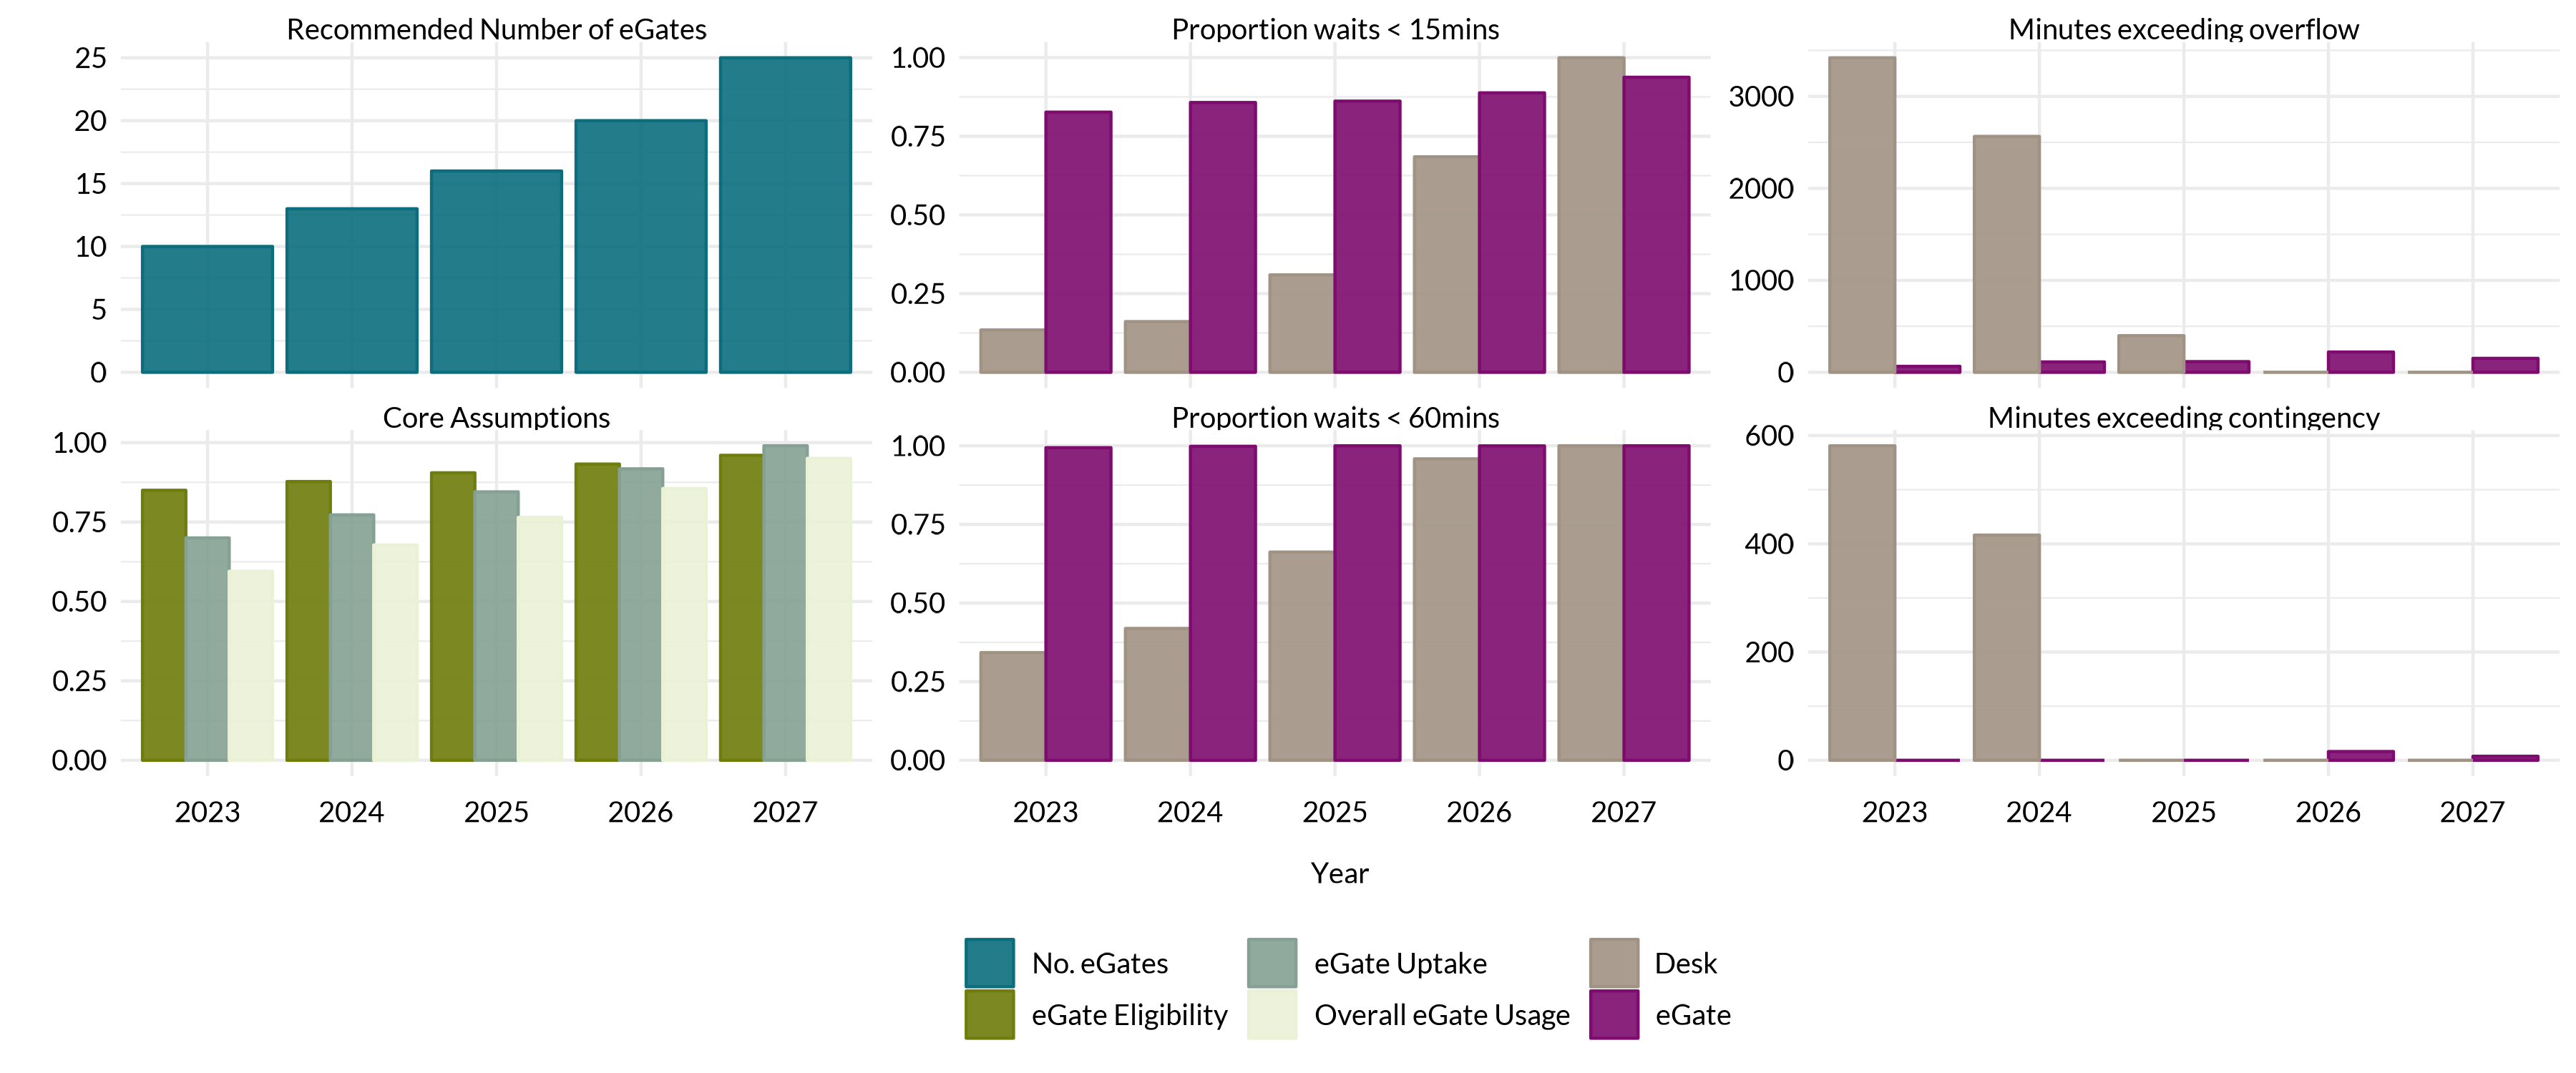
\includegraphics[width=\textwidth]{figures/core_rec_fig.png}
     %\caption{Recommended \glsxtrshort{egate} construction schedule, alongside usage assumptions and \glsxtrshort{kpi} summaries.} \label{fig:core_rec_fig}
\end{figure}

\vspace{-5pt}

We see that excellent \gls{egate} wait times are achievable, and that the main pressure on immigration services comes via queue lengths demanding regular use of the airport's overflow and contingency spaces. This is especially true for desk queues until the airport is able to improve overall \glsxtrshort{egate} usage. We show that measures to change allocation of immigration hall space over time can mitigate this problem, but give extensive evidence that this problem not addressable purely through new \glsxtrshortpl{egate}. 


\begin{tcolorbox}[
colframe=edi-dark-purple,
colback=edi-light-purple,
fonttitle=\bfseries,
title = {Use our Shiny Application to interactively explore demand scenarios!}]
\begin{itemize}
\item URL: \url{https://jacob-bradley.shinyapps.io/shiny/}
\item Username: \texttt{edi-airport} \quad Password: \texttt{flowhost}
\end{itemize}
\end{tcolorbox}


\end{document}